\documentclass{segabs}
\usepackage{xspace,color,amsmath}
\usepackage{amssymb}
\usepackage{hyperref}
\begin{document}
\title{Exploring the influence of various transfer functions on airborne magnetotelluric inversion}
\author{
Devin C. Cowan$^1$, Lindsey J. Heagy$^1$, Douglas W. Oldenburg$^1$ \\
$^1$Geophysical Inversion Facility, University of British Columbia \\
}
\email{devin.cowan@ubc.ca}
% \footer{Example}
\lefthead{Cowan, Heagy \& Oldenburg}
\righthead{Influence of transfer functions on airborne magnetotelluric inversion}
\maketitle

\begin{abstract}

\vspace{-15pt}
Airborne magnetotelluric (AirMT) systems generate transfer function data from magnetic fields measured in the air, and either electric or magnetic fields measured at a base station. The data collected during an AirMT survey is system-dependent and can be generated using one or more directional components of the magnetic field measured in the air. Data collected by various AirMT systems may not produce the same diagnostic anomalies, and may not recover the same conductivity model when inverted using the same inversion hyperparameters. We use numerical forward simulation to analyze the transfer function data that can be generated from 3-component airborne magnetic field measurements. Our analysis indicates that the shape, amplitude and/or phase of AirMT anomalies can be measurably influenced by 3D structure at the base station, regardless of whether data are collected using an electric or magnetic base station. We invert AirMT data to recover a conductivity model using four separate sets of transfer function data, where all inversions use identical hyperparameters. For a remote base station, the locations and depths of structures within the region of interest are recovered consistently for all sets of transfer functions. However different transfer function data, when inverted, may recover different structures within the region of interest and/or near the base station.
\end{abstract}

\vspace{-15pt}
\section{Introduction}
\vspace{-5pt}
Magnetotelluric (MT) methods have long been used to characterize the distribution of subsurface electrical conductivities \citep{Tikhonov1950, Cagniard1953, Ward1959, Vozoff1972}. MT surveys collect impedance and/or tipper data, which define transfer functions that relate directional components of the Earth's natural source electric and magnetic fields. Impedance data, which relate horizontal electric and horizontal magnetic fields, can be interpreted directly to infer subsurface conductivity. Impedance data $Z_{ij}$ are defined according to a 2x2 tensor \citep{ChaveJones2012}:
\begin{equation}
\label{eq:impedance_definition}
\begin{bmatrix} Z_{xx} & Z_{xy} \\ Z_{yx} & Z_{yy} \end{bmatrix}
\begin{bmatrix} H_x^{(x)} & H_x^{(y)} \\ H_y^{(x)} & H_y^{(y)} \end{bmatrix} =
\begin{bmatrix} E_x^{(x)} & E_x^{(y)} \\ E_y^{(x)} & E_y^{(y)} \end{bmatrix}
\end{equation}
where superscripts (x) and (y) represent fields produced by 2 incident planewave polarizations. Tipper data, which relate horizontal and vertical magnetic fields, are sensitive to conductivity contrasts across vertical interfaces. Tippers $T_{zx}$ and $T_{zy}$ are defined according to \citep{ChaveJones2012}:
\begin{equation}
\label{eq:tipper_definition}
\begin{bmatrix} H_z^{(x)} \\ H_z^{(y)} \end{bmatrix} =
\begin{bmatrix} H_x^{(x)} & H_y^{(x)} \\ H_x^{(y)} & H_y^{(y)} \end{bmatrix}
\begin{bmatrix} T_{zx} \\ T_{zy} \end{bmatrix}
\end{equation}
Airborne magnetotelluric (AirMT) systems were developed to rapidly collect MT-like data over large areas and in regions where ground MT surveys are infeasible. AirMT systems generate transfer function data from magnetic fields measured in the air, and either electric or magnetic fields measured at a base station. Z-axis Tipper EM (ZTEM) data are acquired by measuring vertical magnetic fields in the air and horizontal magnetic fields at a base station \citep{LoZang2008}. Quantum Audio Magnetotelluric (QAMT) data are acquired by measuring 3-component magnetic fields in the air and horizontal electric fields at a base station \citep{Larnier2021}. MobileMT measures the magnetic field amplitude in the air and horizontal electric fields at the base station \citep{Sattel2019}.

AirMT data can be inverted to infer the distribution of subsurface conductivities \citep{Holtham2010,Sattel2019}. The structures that are recovered using inversion are greatly influenced by sensitivity functions, which quantify the relationship between the data and the model parameters. For AirMT inversion, the sensitivity functions are dependent on the transfer function data being inverted and the locations of the receivers relative to subsurface structures. Data collected using various AirMT survey configurations may not recover the same conductivity model, even if identical hyperparameters are used in the inversion. Since AirMT data are computed by combining fields measured at separate locations, AirMT inversion can fit the data by placing structures within the region of interest (ROI) and/or near the base station. Our motivation is to better understand the structures that are recovered from AirMT inversion.

In this abstract, we define the fundamental set of AirMT transfer function data that can be collected for both electric and magnetic base stations. Using numerical forward simulation, we analyze how AirMT anomalies for different transfer functions are influenced by a 3D structure at the base station. For several survey configurations, which collect different combinations of transfer function data, we demonstrate how the conductivities recovered using geophysical inversion may differ.
\vspace{-20pt}
%========================================================
\section{Fundamental AirMT Transfer Functions}
%========================================================
\vspace{-5pt}
Here, we define the fundamental set of AirMT transfer functions for both electric and magnetic base stations. For AirMT data collected using a magnetic base station, we extend the tipper relationship in equation \ref{eq:tipper_definition} to include horizontal airborne magnetic field measurements:
\begin{equation}
\label{eq:tipper_definition_ext}
\begin{bmatrix}\! H_x^{(x)} &\! H_y^{(x)} &\! H_z^{(x)} \\ \! H_x^{(y)} & \! H_y^{(y)} & \! H_z^{(y)} \end{bmatrix}_r \!\!\!\!\! = \!\!
\begin{bmatrix}\! H_x^{(x)} &\! H_y^{(x)} \\ \! H_x^{(y)} & \! H_y^{(y)} \end{bmatrix}_b \!
\begin{bmatrix}\! T_{xx} &\! T_{yx} & \! T_{zx} \\ \! T_{xy} & \! T_{yy} & \! T_{zy} \end{bmatrix}
\end{equation}
where the subscript $r$ denotes roving airborne field measurements and subscript $b$ denotes fields measured at a ground base station. $T_{zx}$ and $T_{zy}$ are tipper data, which map the anomalous vertical magnetic fields produced by 3D structures \citep{Vozoff1972}. $T_{xx}$, $T_{xy}$, $T_{yx}$ and $T_{yy}$ map the anomalous horizontal magnetic fields. Note that for a 1D layered Earth, $T_{xy}, T_{yx}, T_{zx}, T_{zy}$ = 0 and $T_{xx}, T_{yy}$ = 1. In this case, no diagnostic information is collected about the subsurface conductivity.

We cannot directly extend the impedance relationship in equation \ref{eq:impedance_definition} to include vertical airborne magnetic fields, as computation of these transfer functions would require the inverse of a 3x2 matrix. Instead, transfer functions for an electric base station are defined according to the admittance relationship:
\begin{equation}
\label{eq:admittance_definition_ext}
\begin{bmatrix} \! H_x^{(x)} & \! H_y^{(x)} & \! H_z^{(x)} \\ \! H_x^{(y)} & \! H_y^{(y)} & \! H_z^{(y)} \end{bmatrix}_r \!\!\!\! = \!
\begin{bmatrix} \! E_x^{(x)} & \! E_y^{(x)} \\ \! E_x^{(y)} & \! E_y^{(y)} \end{bmatrix}_b
\begin{bmatrix} \! Y_{xx} & \! Y_{yx} & \! Y_{zx} \\ \! Y_{xy} & \! Y_{yy} & \! Y_{zy} \end{bmatrix}
\end{equation}
Like tippers, $Y_{zx}$ and $Y_{zy}$ map the anomalous vertical magnetic fields produced by 3D structures. $Y_{xx}$, $Y_{xy}$, $Y_{yx}$ and $Y_{yy}$ map the anomalous horizontal magnetic fields. Transfer functions $Y_{ij}$ are scaled proportional to the inverse of the horizontal electric fields measured at the base station. Consequently, transfer functions $Y_{ij}$ are directly sensitive to the conductivity at the base station. Note that for a 1D layered Earth, the transfer functions in equation \ref{eq:admittance_definition_ext} reduce to $Y_{xx}, Y_{yy}, Y_{zx}, Y_{zy}$ = 0, $Y_{xy}$ = $Z_{yx}^{-1}$, and $Y_{yx}$ = $Z_{xy}^{-1}$. $Z_{xy}$ and $Z_{yx}$ are defined in equation \ref{eq:impedance_definition}. We refer to $Y_{xx}$, $Y_{xy}$, $Y_{yx}$ and $Y_{yy}$ as ``quasi-admittances" since they are computed from fields measured at separate locations.
\begin{figure}[b!]
\centering
\vspace{-10pt}
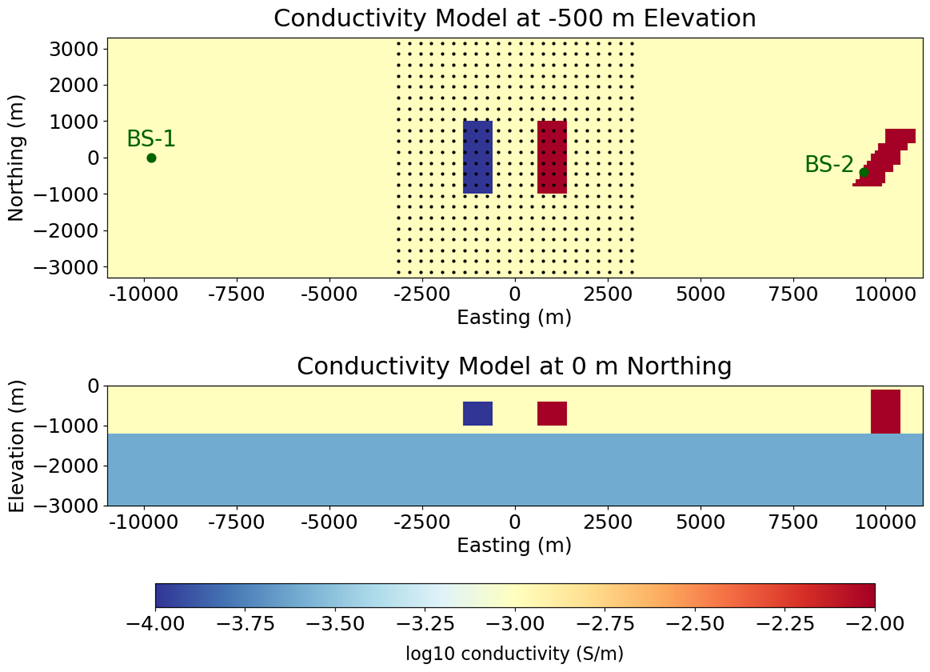
\includegraphics[width=\columnwidth]{images/geology.png}
\vspace{-20pt}
\caption{Problem geometry.}
\label{fig:geology}
\vspace{-5pt}
\end{figure}

\vspace{-12pt}
%========================================================
\section{Influence of Base Station Structures on \\AirMT Anomalies}
%========================================================
\vspace{-8pt}
\label{sec:anomalies}
Here, we analyze the influence of a 3D structure at the base station on AirMT anomalies. We consider the problem geometry in Figure \ref{fig:geology}, wherein a conductor and a resistor are buried within a layered Earth. SimPEG \citep{Cockett2015} is used to simulate natural source electromagnetic fields and AirMT data for base stations at two remote locations. Base station 1 (BS-1) is located over a 1D layered Earth (Easting = -9,800 m and Northing = 0 m). Base station 2 (BS-2) is located over the edge of a conductive dyke (Easting = 9,400 m, Northing = -400 m). Data are simulated using a $+i\omega t$ Fourier convention with X = Easting, Y = Northing and Z positive upward. Outputs are used to quantify how the existence of the conductive dyke near the base station influences AirMT anomalies.

\subsection{Simulated Anomalies}
\label{sec:anomalies}
\vspace{-8pt}

In Figure \ref{fig:tipper_anomalies}, we illustrate the differences between simulated $T_{zy}$ anomalies at 270 Hz for magnetic base stations located at BS-1 and BS-2. Tipper data are considered to be minimally sensitive to subsurface conductivity at the base station. However, the conductive dyke near BS-2 introduces a scaling to the data values that reduces the anomaly amplitudes by $\sim$10 \%. The irregular features illustrated in Figures \ref{fig:tipper_anomalies}c and \ref{fig:tipper_anomalies}f also indicate a measurable difference in anomaly shape.

In Figure \ref{fig:admittance_anomalies}, we illustrate the differences between simulated $Y_{yx}$ anomalies at 270 Hz for electric base stations located at BS-1 and BS-2. Here, the conductive dyke near BS-2 introduces a scaling that increases the amplitudes of the real components by $\sim$40 \% and the imaginary components by $\sim$ 70\%. The irregular features illustrated in Figures \ref{fig:admittance_anomalies}c and \ref{fig:admittance_anomalies}f indicate a measurable difference in anomaly shape. The phase relationship between the real and imaginary components of $Y_{yx}$ is also influenced. For data simulated using BS-1, the real components of $Y_{yx}$ are larger in magnitude than the imaginary components (Figures \ref{fig:admittance_anomalies}a and \ref{fig:admittance_anomalies}d). For data simulated using BS-2, the real components of $Y_{yx}$ are smaller in magnitude than the imaginary components (Figures \ref{fig:admittance_anomalies}b and \ref{fig:admittance_anomalies}e).


\subsection{Quantifying the Influence of the Base Station}

To understand the differences between our simulated AirMT anomalies, we develop mathematical relationships for quantifying the impact the base station location. For AirMT data simulated for a magnetic base station, let $\mathbf{H}(b_1)$ and $\mathbf{H}(b_2)$ be 2x2 matrices that define the horizontal magnetic fields measured at BS-1 and BS-2, respectively. The relative distortion between $\mathbf{H}(b_1)$ and $\mathbf{H}(b_2)$ due to the conductive dyke can be characterized by a 2x2 matrix $\mathbf{A}_{12}$, such that:
\begin{equation}
\label{eq:base_relationship}
\mathbf{H}(b_2) \, \mathbf{A}_{12} = \mathbf{H}(b_1)
\end{equation}
Using Equations \ref{eq:tipper_definition_ext} and \ref{eq:base_relationship}, we obtain:
\begin{equation}
\label{eq:distortion_h}
\begin{split}
\mathbf{H}(r) &= \mathbf{H}(b_1) \, \mathbf{T}(r, b_1) = \mathbf{H}(b_2) \, \mathbf{T}(r, b_2)\\
&\implies \mathbf{T}(r, b_2) = \mathbf{A}_{12} \, \mathbf{T}(r, b_1)
\end{split}
\end{equation}
where $\mathbf{H}(r)$ represents the roving airborne magnetic field measurements. From equation \ref{eq:distortion_h}, any distortion of the horizontal fields measured at a magnetic base station corresponds directly to a distortion of the transfer function data.
Using SimPEG, we simulate the fields for $\mathbf{H}(b_1)$ and $\mathbf{H}(b_2)$. We compute the entries of $\mathbf{A}_{12}$ by applying the inverse of $\mathbf{H}(b_2)$ to $\mathbf{H}(b_1)$. For an operating frequency of 270 Hz, we obtain:
\begin{equation}
\label{eq:distortion_h_computed}
\mathbf{A}_{12} = \begin{bmatrix}
0.922+0.009 \, i & 0.065 - 0.008 \, i \\
0.049- 0.006 \, i & 0.891+ 0.008 \, i
\end{bmatrix}
\end{equation}
The influence of the conductive dyke on the amplitude of the $T_{ij}$ anomalies can be understood by examining the square root of the amplitude of the determinant of $\mathbf{A_{12}}$. Here, $\sqrt{|det(\mathbf{A_{12}})|}$ = 0.904 indicates a $\sim$10 \% reduction in anomaly amplitude. Non-zero off-diagonal entries within $\mathbf{A_{12}}$ indicate rotation of the $T_{ij}$ anomalies. Since the off-diagonal entries are much smaller in amplitude than the diagonal entries, we expect the shapes of $T_{ij}$ anomalies to be minimally impacted. $\mathbf{A_{12}}$ contains complex numbers, indicating the phase of the data are influenced. Here, the imaginary components are very small, indicating a negligible distortion of the phase. Our analysis of equation \ref{eq:distortion_h_computed} is consistent with our analysis of simulated AirMT data in Figure \ref{fig:tipper_anomalies}.
\begin{figure}[t!]
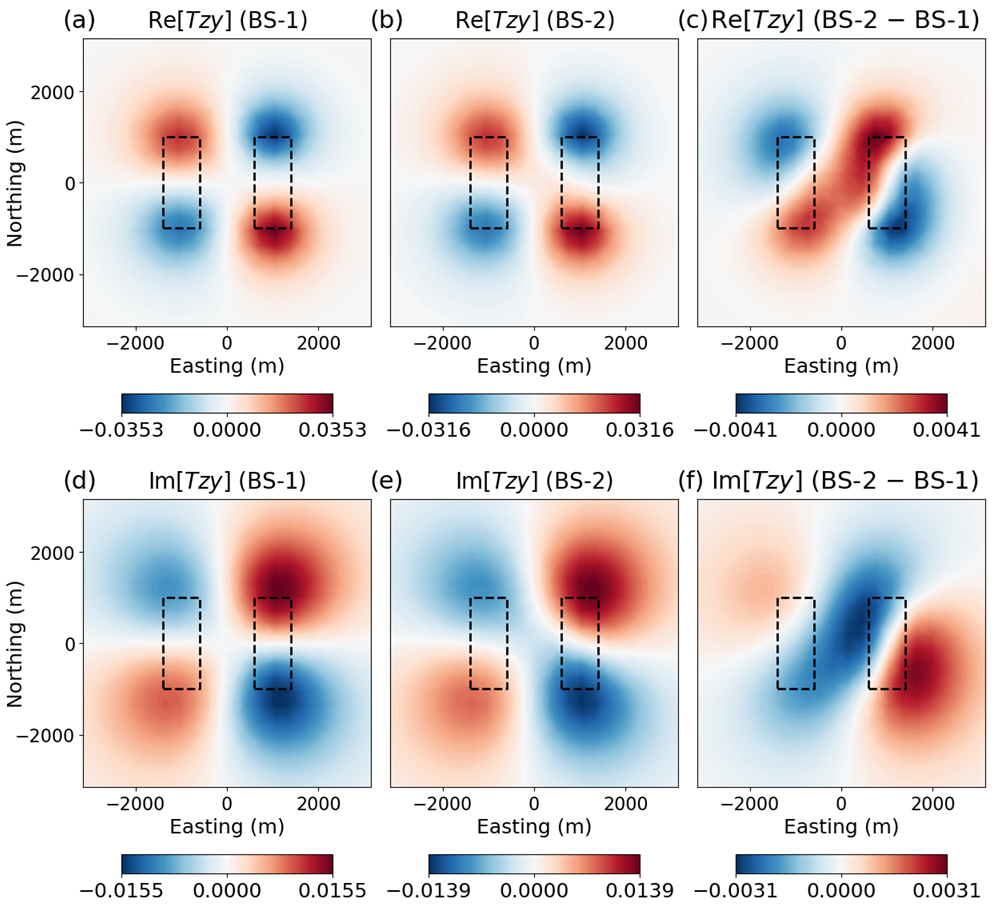
\includegraphics[width=\columnwidth]{images/anomalies_tipper.png}
\vspace{-20pt}
\caption{Comparison between $T_{zy}$ simulated at 270 Hz for BS-1 and BS-2.}
\label{fig:tipper_anomalies}
\vspace{10pt}
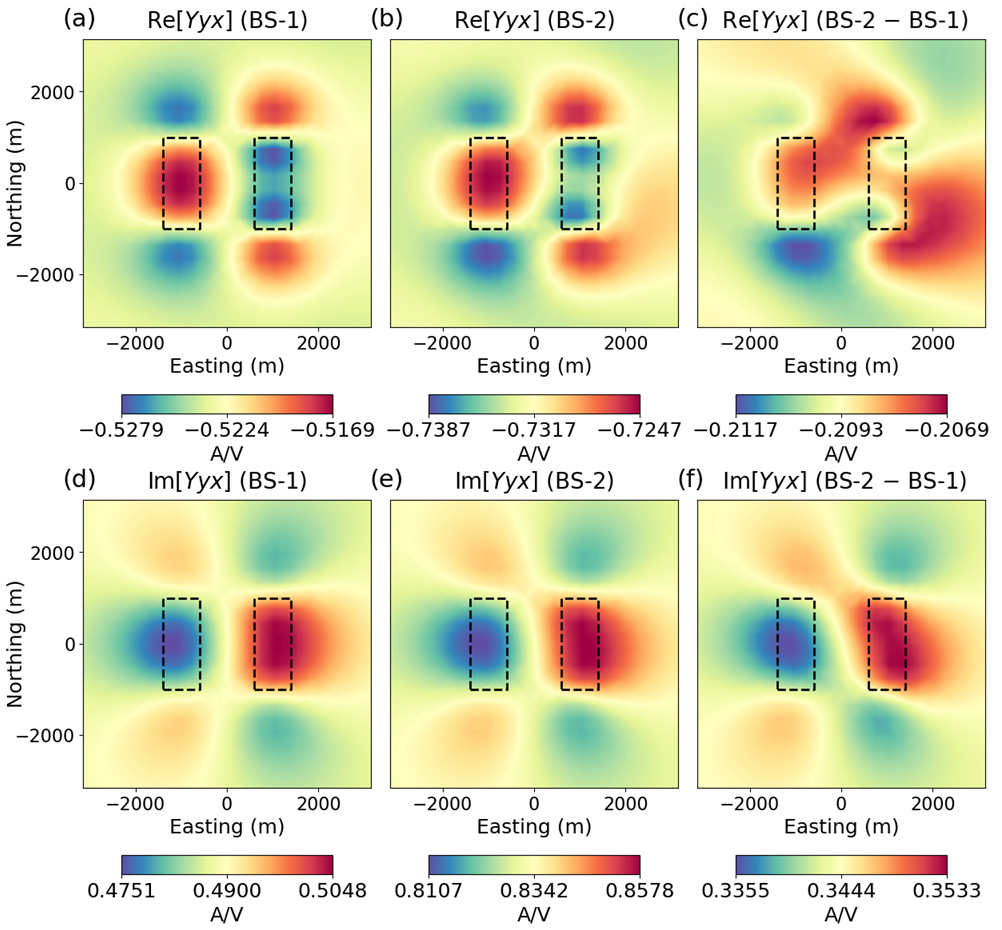
\includegraphics[width=\columnwidth]{images/anomalies_admittance.png}
\vspace{-20pt}
\caption{Comparison between $Y_{yx}$ simulated at 270 Hz for BS-1 and BS-2.}
\label{fig:admittance_anomalies}
\vspace{-10pt}
\end{figure}

Now let $\mathbf{E}(b_1)$ and $\mathbf{E}(b_2)$ be 2x2 matrices that define the horizontal electric fields measured at BS-1 and BS-2, respectively. We define the relative distortion between $\mathbf{E}(b_1)$ and $\mathbf{E}(b_2)$ according to:
\begin{equation}
\label{eq:base_relationship_2}
\mathbf{E}(b_2) \, \mathbf{B}_{12} = \mathbf{E}(b_1)
\end{equation}
where $\mathbf{B}_{12}$ is the 2x2 distortion matrix. Using equations \ref{eq:admittance_definition_ext} and \ref{eq:base_relationship_2}, the existence of the conductive dyke distorts the quasi-admittances according to:
\begin{equation}
\mathbf{Y}(r, b_2) = \mathbf{B}_{12} \, \mathbf{Y}(r, b_1)
\end{equation}
Thus any distortion of the horizontal fields measured at an electric base station corresponds directly to a distortion of the transfer function data. For an operating frequency of 270 Hz, the entries of $\mathbf{B}_{12}$ for our problem geometry yield:
\begin{equation}
\label{eq:distortion_e_computed}
\mathbf{B}_{12} = \begin{bmatrix}
1.542 - 0.151 \, i & -0.077 + 0.025 \, i \\
-0.105 + 0.092 \, i & 1.629 - 0.343 \, i
\end{bmatrix}
\end{equation}
Here, $\sqrt{|det(\mathbf{B_{12}})|} = 1.603$ indicates a $\sim$60 \% increase in the amplitudes of the data values. $\mathbf{B}_{12}$ contains off-diagonal entries which are much smaller in amplitude than the diagonal entries, implying rotation of the AirMT anomalies is minimally significant. The entries of $\mathbf{B_{12}}$ have significant imaginary components, indicating an observable impact on the phase of the data values. Our analysis of equation \ref{eq:distortion_e_computed} is consistent with our analysis of simulated AirMT data in Figure \ref{fig:admittance_anomalies}.

\vspace{-15pt}
%========================================================
\section{Inversion of AirMT Data}
%========================================================
\vspace{-5pt}
\subsection{Methodology}

For the conductivity model illustrated in Figure \ref{fig:geology}, the influence of various transfer functions on AirMT inversion is analyzed. Synthetic AirMT data at 30 Hz, 90 Hz, 270 Hz and 720 Hz are generated for BS-2. Gaussian random noise is added to each dataset. We use SimPEG \citep{Cockett2015} to invert four datasets, each of which corresponds to a different set of transfer function data. Our data sets include:

$\bullet$ $T_{zx}$ and $T_{zy}$: Roving $H_z$, and a magnetic base station.\\
$\bullet$ $Y_{zx}$ and $Y_{zy}$: Roving $H_z$, and an electric base station.\\
$\bullet$ $T_{xy}$, $T_{xy}$, $T_{yy}$ and $T_{yy}$: Roving $H_x$ and $H_y$, and a magnetic base station. \\
$\bullet$ $Y_{xy}$, $Y_{xy}$, $Y_{yy}$ and $Y_{yy}$: Roving $H_x$, and $H_y$, and an electric base station.

\begin{figure*}[t!]
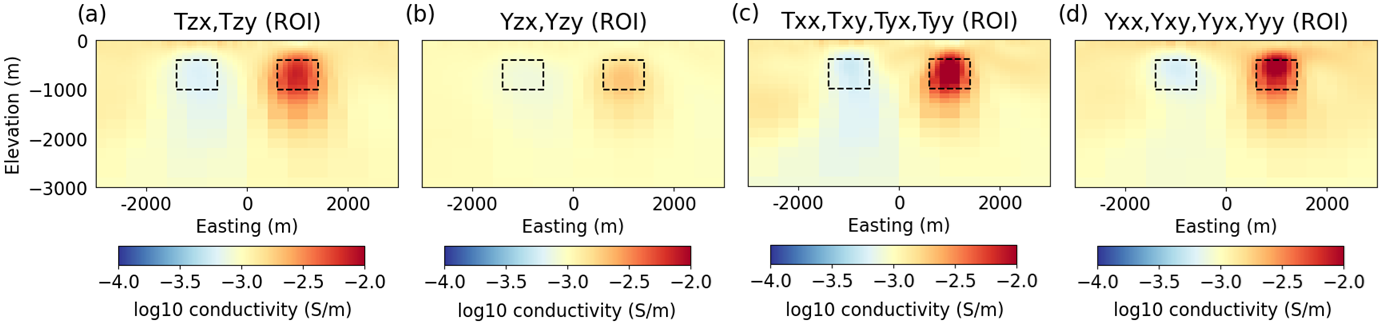
\includegraphics[width=2\columnwidth]{images/inversion.png}
\vspace{-8pt}
\caption{Inversion models within the region of interest (ROI), recovered from AirMT data using different survey configurations. All models are plotted on the same color scale. (a) $T_{zx}$, $T_{zy}$. (b) $Y_{zx}$, $Y_{zy}$. (c) $T_{xx}$, $T_{xy}$, $T_{yx}$, $T_{yy}$. (d) $Y_{xx}$, $Y_{xy}$, $Y_{yx}$, $Y_{yy}$.}
\label{fig:inversion}
\vspace{5pt}
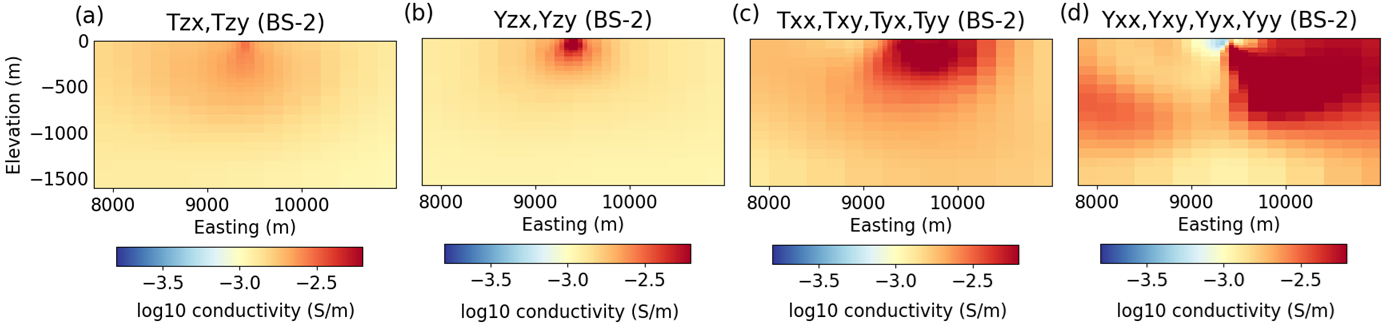
\includegraphics[width=2\columnwidth]{images/inversion_base.png}
\vspace{-6pt}
\caption{Recovered structures at the base station (BS-2). All models are plotted on the same color scale. (a) $T_{zx}$, $T_{zy}$. (b) $Y_{zx}$, $Y_{zy}$. (c) $T_{xx}$, $T_{xy}$, $T_{yx}$, $T_{yy}$. (d) $Y_{xx}$, $Y_{xy}$, $Y_{yx}$, $Y_{yy}$.}
\label{fig:inversion_base}
\vspace{-15pt}
\end{figure*}
For each dataset, we recover the model ($\mathbf{m}$) that minimizes an objective function of the form:
\begin{equation}
\arg \min_\mathbf{m} \; \phi_d (\mathbf{m}) + \beta \, \phi_m (\mathbf{d})
\end{equation}
The data misfit $\phi_d (\mathbf{m})$ is given by:
\begin{equation}
\phi_d (\mathbf{m}) = \sum_{i=1}^{nD} \; \Bigg ( \frac{d_i^{(pre)} - d_i^{(obs)} }{\varepsilon_i} \Bigg )^2
\end{equation}
The model objective function $\phi_m (\mathbf{m})$, which penalizes structure in the recovered model, is given by:
\begin{equation}
\phi_m (\mathbf{m}) = \alpha_s \big \| \mathbf{m - m}^{(ref)} \big \|^2 + \sum_{k=x,y,z} \alpha_k \big \| \mathbf{G_k \, m} \big \|^2
\end{equation}
$\beta$ is the trade-off parameter which balances the data misfit and model objective function. We set hyperparameters $\alpha_s$ = 1e-8 and $\alpha_x,\alpha_y, \alpha_z=1$ to recover the smoothest model. The true host conductivity of 1e-3 S/m is used as the starting and reference model in the inversion, representing a``best-case" scenario.
%We will not analyze the impact of the starting model on AirMT inversion.

%========================================================
\subsection{Inversion Results}
%========================================================

For each inversion, the structures recovered within the ROI are illustrated in Figure \ref{fig:inversion}. For all datasets, the locations and depths of the conductor and the resistor are recovered consistently. We observe some variability in the margins of the recovered resistor at depth. The conductivity contrasts between recovered structures and the host differs between the different datasets. Recovered conductivity contrasts appear underestimated when inverting transfer function data generated using vertical airborne magnetic field measurements. This is especially true when electric fields are measured at the base station (Figure \ref{fig:inversion}b).

Differences in the recovered models in Figure \ref{fig:inversion} can be understood by analyzing the structures recovered at the base station, which we show in Figure \ref{fig:inversion_base}. From Figure \ref{fig:inversion_base}, it is clear that the structures recovered at the base station are highly dependent on the transfer functions that are used in the inversion. For transfer function data generated using vertical airborne magnetic field measurements, we recover more localized structure at the base station. From Figures \ref{fig:inversion}b and \ref{fig:inversion_base}b, we determined that the structure recovered at the base station was primarily responsible for scaling the amplitudes of the predicted data anomalies in $Y_{zx}$ and $Y_{zy}$. That is, the inversion places structure at the base station instead of recovering larger conductivity contrasts within the ROI. This behavior is also exhibited when inverting $T_{zx}$ and $T_{zy}$ data (Figures \ref{fig:inversion}a and \ref{fig:inversion_base}a), however, the behavior is significantly diminished since the fields measured at a magnetic base station is much less sensitive to subsurface conductivity.

For transfer function data generated using horizontal airborne magnetic field measurements, significant structure is recovered at the base station regardless of the fields that are measured there (Figures \ref{fig:inversion_base}c and \ref{fig:inversion_base}d). However, the conductivity contrasts for the recovered conductor and resistor are comparable to the conductivity contrasts in the true model.
\vspace{-10pt}
%========================================================
\section{Conclusions}
%========================================================
\vspace{-5pt}
We demonstrated that a 3D structure near the base station can measurably influence the shape, amplitude and/or phase of\\ AirMT anomalies, regardless of the fields that are measured at the base station. This influence is greater for systems which measure electric fields at the base station. For the problem geometry used in our analysis, the presence of a 3D structure at the base station primarily influences the amplitudes of the data values. Further analysis is needed to determine whether the orientation of AirMT anomalies and/or phase of AirMT data are consistently more robust to 3D structure at the base station.

Analysis of smoothest model inversion results indicates that recovered conductivity models depend on the transfer functions that are collected. Inversion of AirMT data for various survey configurations yielded variability in the structures that are recovered within the ROI and near the base station. For the problem geometry used in our analysis, the location and horizontal margins of structures recovered within the ROI were generally consistent. For AirMT data generated using vertical airborne magnetic field measurements, the recovered models can underestimate conductivity contrasts within the ROI. 

Further analysis is required to understand how structure recovered at the base station contributes to fitting AirMT data. The extent to which AirMT inversion may fit the observed data by recovering erroneous structure at the base station could be investigated by comparing the observed and predicted magnetotelluric fields at the base station. Improvements to AirMT methods may be obtained by exploring improvements to the survey design. The analysis provided in our abstract did not consider a base station located within the ROI. Future analysis may determine whether collecting AirMT data using multiple base stations and/or collecting both electric and magnetic fields at base stations provide added benefit. 

% For bibliography
\onecolumn
\bibliographystyle{seg} % style file is seg.bst
\bibliography{bibliography}
\end{document}




